\chapter{Introduction}
This dissertation concerns the design and development of a secure development and testing tool for \gls{mcp} implementations. The work sits within the field of Generative Artificial Intelligence applied to cybersecurity, with particular emphasis on identifying, analyzing, and mitigating emerging threats in \gls{llm}-driven systems that interact with external tools and services.

This chapter is organized as follows. Section~\ref{sec:motivation} describes the problem domain and the relevance of \gls{mcp} security. Section~\ref{sec:objectives} states the objectives, the research question, and the expected contributions. Section~\ref{sec:method} presents the research method that guided the work. Section~\ref{sec:structure} outlines the remaining chapters.

\section{Motivation}
\label{sec:motivation}

The integration of \glspl{llm} into enterprise systems has changed how \gls{ai} interacts with real-world environments. Modern AI applications no longer operate in isolation. They retrieve contextual information, invoke external tools, interact with \glspl{api}, and communicate with other autonomous agents. The \gls{mcp} was introduced to formalize and standardize these interactions, enabling structured communication between AI models and external systems \citep{anthropic2024mcp}.

While \gls{mcp} enhances AI capabilities, it also introduces a new and complex attack surface. Traditional cybersecurity mechanisms were not designed to address vulnerabilities that arise from natural-language interactions, autonomous tool execution, or \gls{a2a} communication. MCP-enabled systems are exposed to \gls{prompt_injection} \citep{greshake2023prompt, liu2024universal}, privilege escalation, unauthorized data access, tool misuse, and cascading agent compromise.

As enterprises and critical infrastructures adopt MCP-based architectures, the need for a security-first development approach grows with them. Existing secure coding guidelines and testing methodologies fall short for \gls{llm}-driven systems \citep{owasp2024llm}, because they do not account for context manipulation, adversarial prompting, or emergent behavior in multi-agent environments. This work is therefore motivated by the need for an automated, security-oriented development and testing tool tailored specifically to MCP implementations, one that reduces systemic risk while supporting safe and scalable adoption of AI-integrated systems.

\section{Objectives and Research Question}
\label{sec:objectives}

The central research question is:

\begin{quote}
\textit{Can the security posture of a Model Context Protocol server be assessed automatically, both from its running interface and from its source code, using language models to reason about an attack surface that is not known in advance?}
\end{quote}

To answer it, this work develops a security tool for MCP servers and \gls{llm}-based applications that integrates automated vulnerability detection, a reusable vulnerability taxonomy, structured remediation guidance, and repeatable, scriptable scans with a durable history of results. A central component is an \gls{llm}-assisted analysis pipeline capable of:

\begin{itemize}
    \item analyzing MCP implementations for structural and semantic security flaws;
    \item performing \gls{static_analysis} on MCP server source code;
    \item conducting dynamic adversarial testing using crafted prompts and malicious inputs;
    \item testing tool permission boundaries and access control under a low-privilege session;
    \item producing remediation recommendations aligned with established cybersecurity principles and emerging AI threat patterns, together with a \gls{cvss} v3.1 severity score and \gls{cia} impact for every finding.
\end{itemize}

The expected contribution is twofold. First, a working artifact that unifies dynamic testing and static analysis of MCP servers under a single vulnerability taxonomy and a single remediation catalog. Second, a set of design decisions and observations, including the handling of untrusted tool descriptions during automated triage, that inform secure development practice for this ecosystem.

\section{Research Method}
\label{sec:method}

The work follows the \gls{dsr} methodology \citep{hevner2004design}, which is suited to problems whose solution is the design, implementation, and rigorous evaluation of an artifact that addresses a concrete, unsolved problem in a real-world domain. Here the problem is the absence of a structured, security-focused development and testing tool specifically for \gls{mcp} implementations: existing tools cover parts of the space but do not combine protocol-level threat analysis, automated vulnerability detection, adversarial testing, and secure development guidance in one place. Figure~\ref{fig:dsr_methodology} summarizes the process and the iterative relationship between its stages.

\begin{figure}[htbp]
    \centering
    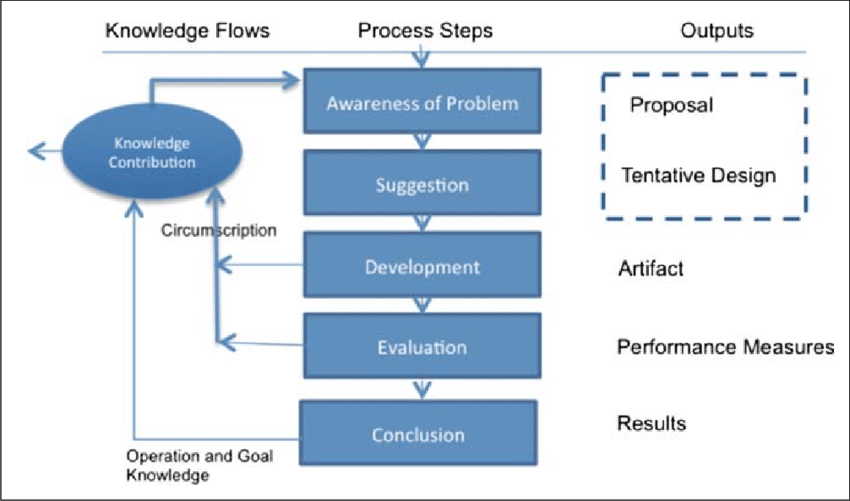
\includegraphics[width=\linewidth]{images/dsr.png}
    \caption{Design Science Research process (adapted from \citep{hevner2004design}).}
    \label{fig:dsr_methodology}
\end{figure}

The research was structured into five stages aligned with the \gls{dsr} cycle. Problem identification and threat analysis examined the \gls{mcp} specification to locate attack-surface expansion, trust boundaries, and protocol-level weaknesses, including \gls{threat_modeling} of client-server interactions, tool invocation, and agent-to-agent flows \citep{qi2025protocol}. The definition of security requirements then translated those weaknesses into functional and non-functional requirements that guide the architecture and establish measurable evaluation criteria \citep{nist2022ssdf, nist2020zerotrust}. Artifact design and development produced the tool itself, combining static analysis of server source, dynamic adversarial testing, testing of tool permission boundaries, and detection of potential data-leakage paths. Demonstration applies the artifact to controlled MCP environments and representative implementation scenarios, with adversarial cases simulating realistic attack patterns \citep{greshake2023prompt, owasp2024llm01}. Evaluation then assesses the tool against qualitative and quantitative criteria; this final stage is reported in Chapter~\ref{chap:results}.

\section{Document Structure}
\label{sec:structure}

The remainder of this dissertation is organized into five chapters. Chapter~\ref{chap:background} presents the theoretical framework, covering \glspl{llm}, the Model Context Protocol, and the cybersecurity concepts that underpin the work. Chapter~\ref{chap:architecture} describes the architecture of the proposed solution, including its two analysis paths, the shared taxonomy, and the main design decisions. Chapter~\ref{chap:implementation} details the implementation of each module. Chapter~\ref{chap:results} reports the evaluation, including the test targets, benchmarks, and a discussion of the results. Chapter~\ref{chap:conclusion} concludes and outlines directions for future work.
